\section{Transfer Learning}
Transfer learning is the method of applying a trained model on another dataset with similar traits. One popular application is to use it on image classification on small datasets that have insufficient number of labeled samples. Since deep convolutional networks trained on large-scale datasets learn universal features of images, it is a common practice to use the convolutional layers of the deep network as a feature extractor. Then by retraining the features on a simple single or multi layer network, one can train a image classifier on a small dataset.

\subsection{VGG16 Model}
For our task, we use the VGG16 model. VGG16 is a very deep convolutional network for large scale image recognition proposed in \cite{Simon}. It is a popular network, apart from AlexNet and GoogLeNet. The architecture of the network is shown in Figure \ref{vgg}.
\begin{figure}[H]
	\centering
	\includegraphics[width=8cm]{vgg16.png}%
	\caption{VGG16 Net Diagram \cite{vgg16fig}}
 	\label{vgg}
\end{figure}
The network consists of 16 layers of weights. The first 13 layers are convolutional layers stacked on top of each other. They extract the features of the images. The last 3 layers are linear layers, which is the classifier for the retrieved features.

\subsubsection{Dataset and Setup}
The dataset we are using is the Caltech-256 \cite{caltech}. It consists of 30607 images distributed over 257 classes. We ignore the "clutter" class and use the remaining 256 classes. From the dataset, we extract 40 images per class. 28 images are taken as our test set, the next 4 images are our validation set and the last 8 images are our test set.
 
To train a classifier on this smaller dataset, we substitute the last layer of the model to a 4096x256 linear layer. The previous layers are fixed and no weight updates are performed. 

We use cross-entropy loss function and Adam optimizer to train the new last layer of the model with mini-batch learning. Early stopping is performed with the tolerance of 10 iterations. We also anneal the learning rate with the following equation: 
\begin{equation}
\mu_t = \dfrac{\mu_0}{1+t/T}
\end{equation}

The parameters of our experiments are show in Table \ref{tab-trans1}. The model converges after 10 epochs, with the train accuracy of 90.04\%, validation accuracy of 72.27\% and test accuracy of 75.54\%

\begin{table}[H]
	\caption{Experiment Parameters}
	\centering
	\begin{tabular}{cc}
		\toprule
		%\multicolumn{5}{c}{Part}                   \\
		\cmidrule{1-2}
		Learning rate & 0.001\\
		\midrule
		Tolerance & 10\\
		\midrule
		T & 10\\
		\midrule
		Momentum & 0.9\\
		\midrule
		BatchSize & 32\\
		\bottomrule
	\end{tabular}
	\label{tab-trans1}
\end{table}

\subsubsection{Discussion}
The training results are shown in Figure \ref{fig-trans1}
%\begin{figure}[H]
%	\centering
%	\subfloat[Accuracy among epochs]{\includegraphics[width=6cm]{trans_correct.png}}%
%	\qquad
%	\subfloat[Loss among epochs]{\includegraphics[width=6cm]{trans_loss.png}}\\%
%	\caption{Accuracy and loss over epochs}
%	\label{fig-trans1}
%\end{figure}

\begin{figure}[H]
\centering
\subcaptionbox{Accuracy among epochs}{\includegraphics[width=0.5\textwidth]{trans_correct.png}}%
\subcaptionbox{Loss among epochs}{\includegraphics[width=0.5\textwidth]{trans_loss.png}}\\%
\caption{Accuracy and loss over epochs}
\label{fig-trans1}
\end{figure}



The overall performance of the new model is decent, considering we are only giving the model 28 images per class, with a total amount of 256 classes. 

The train, validation and test accuracy and loss figures are also reasonable. All of them are monotonic and converge to a maximum/minimum value. 

That being said, there are two abnormalities that can be observed in the figure. One is the unusually high train accuracy. We can see that the training accuracy is much higher than the validation and test accuracy. The validation and training loss quickly converges at the 5th epoch, while the training loss is still decreasing. With a small dataset, limited samples per class are shown to the model, thus it is harder to generalize. We can deduce that the model is overfitting on the limited training samples.

Another is the exceptionally higher validation and test accuracy in the first two epochs. Training accuracy is mostly only used to observe if the model is learning the training set and whether it is overfitting. To speed up computation, we estimate the train accuracy after each epoch by taking the average training accuracy over the mini-batches. Thus we do not need an extra forward pass after each epoch, but compute the training accuracy during the back-propagation process. The validation and test accuracy are calculated after each epoch. Thus the train accuracy is not collected from the same model as the validation and test accuracy. But as the model converges, the train accuracy also converges and is a good representation of the training performance. Because the model is learning at a very fast pace, for the first two epochs, the train accuracy is lower than the validation and test accuracy.

\section{Transfer Learning}
\subsection{Visualization}
Normally for convolutional neural network, visualization can be processed by some naive methods.
\begin{itemize}
\item Visualize the feature maps after convolutional block
\item Visualize the filters in the first convolutional block
\end{itemize}

Feature maps describe how neural network understand an image at certain level, and filters represent patterns the neural network tends to find in each layer. There are also other approaches using deconvolutional network and feature evolution mentioned in \cite{zeiler} to get deeper insights, but requiring for large computation cost. Here for simplicity, we just use the naive techniques described before.

\subsubsection{Experiment Setup}
We still used the pruned VGG16 network mentioned in Section 3.1.1. The parameters of the model are all pre-trained. The weights and bias in conv blocks and the first linear layer are copied from the parameters set trained from ImageNet, and the parameters in the last $4096\times 256$ linea layer is acquired from the Caltech-256 dataset, through transfer learning process.

The visualization of the feature maps is depend on input images, as this represents the activation result after the neural network model receiving the input. In practice, we use an image as input, and let neural network do the feedforward process to acquire the activation result. The activation result of a convolutional layer is a tensor with size $K \times W\times H$, where $K$ is the number of filters, and $W$ and $H$ are size of the feature maps. At last, we pick up a subset of feature maps from the first and last convolutional layers, then plot them as heatmaps.

The weights in filters at first layer can be seen as a $3\times K \times W \times H$ tensor, which indicates the input images have 3 channels(RGB), $K$ filters in first layer and will generate feature maps with width of $W$ and height of $H$. For each filter, we can visualize it as a RGB image, which specifies its preference among different color channels. Although we can also visualize filters in layers afterwards, their inputs are not in pixel-place, hence rarely can provide any intuition to us. Therefore we omit this procedure, and only focus on filters in the first convolutional layer.

\subsubsection{Discussion}
First we picked up a specific image (billiards) as input, shown in Figure \ref{fig-input}

\begin{figure}[H]
  \centering
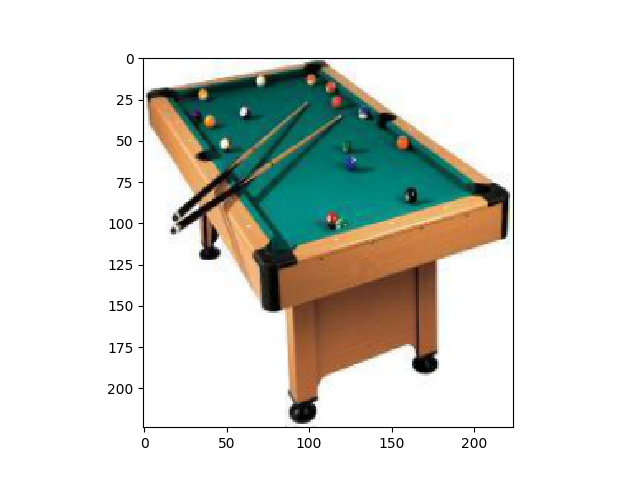
\includegraphics[width=0.5\textwidth]{raw_input.png}
  \caption{The input image}
  \label{fig-input}
\end{figure}

Follows are some results for visualization of activations, represented in headmaps. The activation for the first convolutional layer has size $224\times 224$, whereas the activation for the last convolutional layer has size $14\times 14$. The lighter yellow color indicated strong activation in that area, and the darker blue color means low interest in those regions.

%TODO activation show

\begin{figure}[H]
\centering
\subcaptionbox{from filter 6 (blue vertical line )}{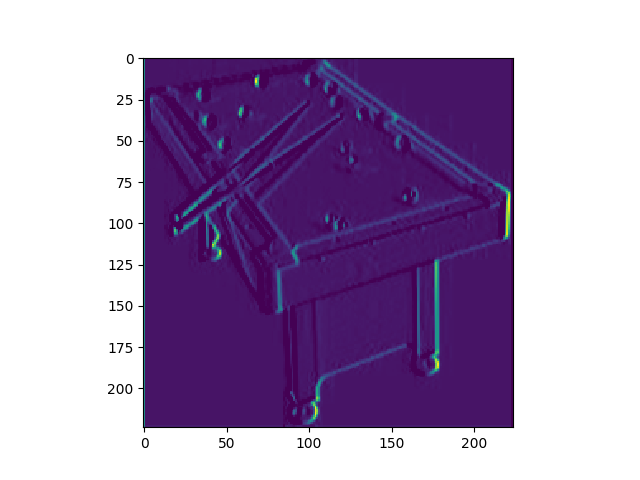
\includegraphics[width=0.5\textwidth]{first_conv6.png}}%
\subcaptionbox{from filter 27 (dark corner)}{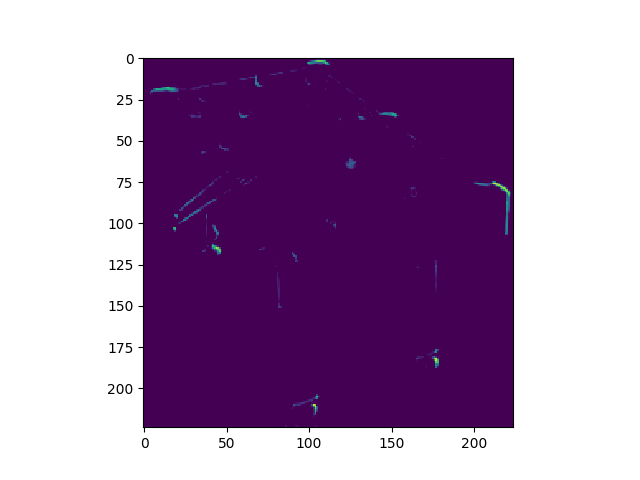
\includegraphics[width=0.5\textwidth]{first_conv27.png}}\\%
\subcaptionbox{from filter 15 (green surface)}{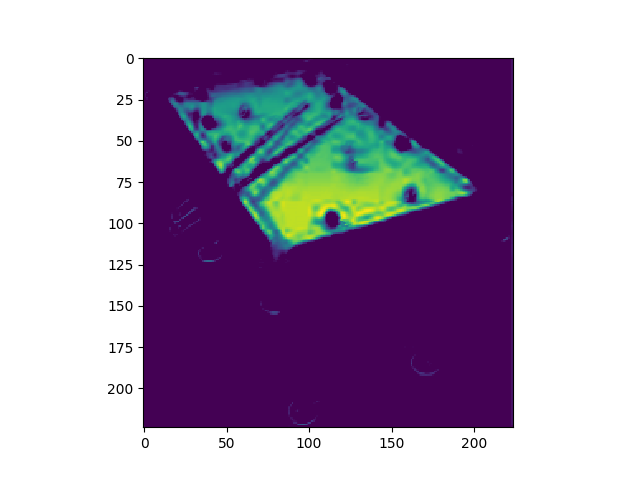
\includegraphics[width=0.5\textwidth]{first_conv15.png}}%
\subcaptionbox{from filter 47 (yellow surface)}{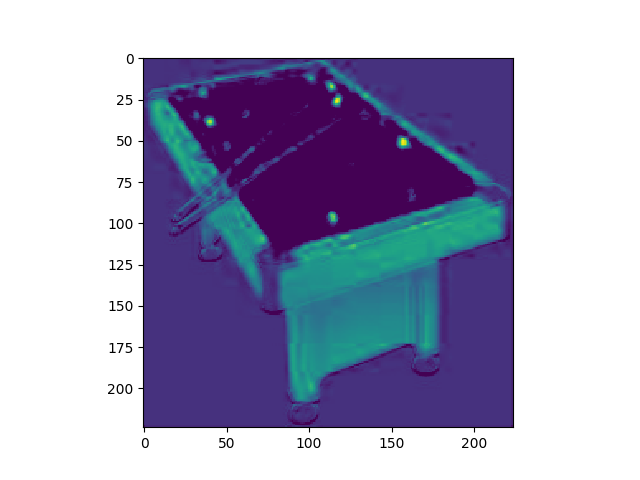
\includegraphics[width=0.5\textwidth]{first_conv47.png}}%
\caption{Activations from different filters in first conv layer}
\label{fig-acti-in}
\end{figure}

We can see that the activations from the first convolutional layer is very illustrated in Figure \ref{fig-acti-in}. The majority of them are just basic geometry feautures extracted by some line detectors(filter 6), corner detectors(filter 27) or texture detectors with repect to differnt colors (compare filter 15 and filter 47). These visualized activation maps are with sharp distinction. While the activations from the last convolutional layer have smaller size and hence are hard to read, shown in Figure \ref{fig-acti-out}. Their inputs are not in pixel-space so we can just infer they are judging some higher-level features from certain interested regions (the contour and content are all blurred, comparing to the first layer activation)

\begin{figure}[H]
\centering
\subcaptionbox{from filter 34 }{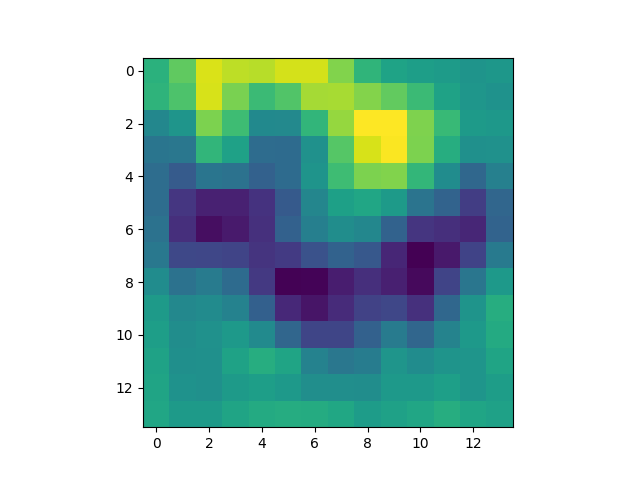
\includegraphics[width=0.25\textwidth]{last_conv34.png}}%
\subcaptionbox{from filter 70}{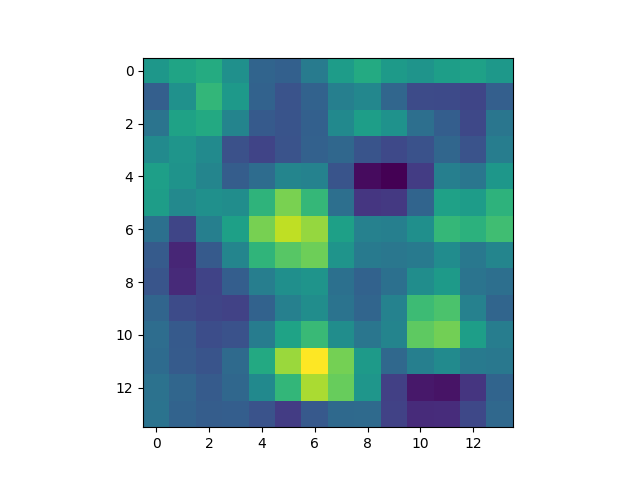
\includegraphics[width=0.25\textwidth]{last_conv70.png}}%
\subcaptionbox{from filter 135}{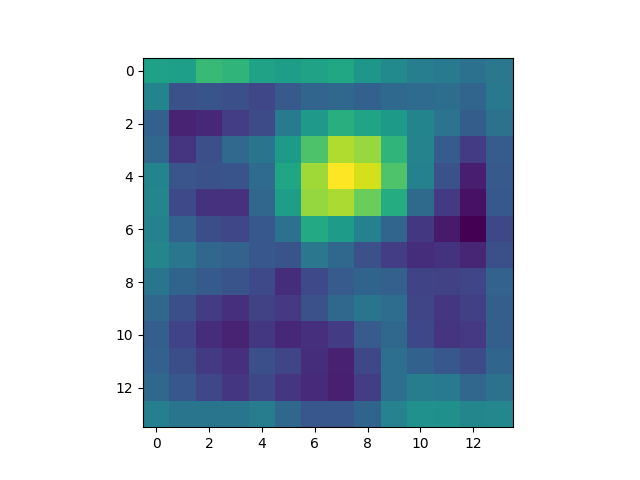
\includegraphics[width=0.25\textwidth]{last_conv135.png}}%
\subcaptionbox{from filter 282}{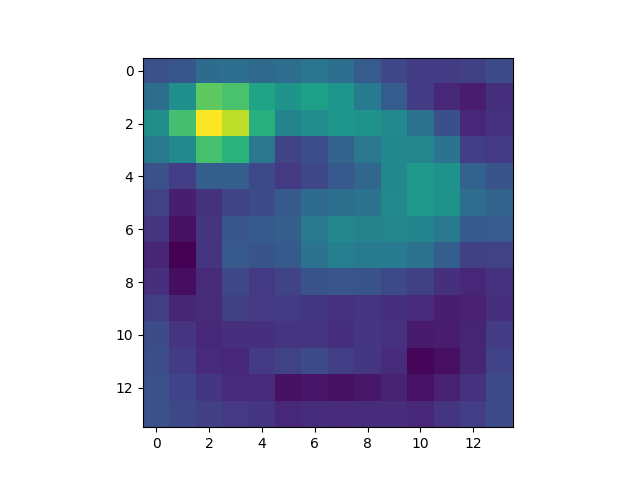
\includegraphics[width=0.25\textwidth]{last_conv282.png}}%
\caption{Activations from different filters in the last conv layer}
\label{fig-acti-out}
\end{figure}


%TODO weights show
%diversity in color and gradient
Then we take a look at the weights of the filters. In Figure\ref{fig-filter-in1} can we see that the diversity of filters in color and gradient of pixel intensity(patterns). It is this diversity to make sure the first layer can extract as much features as possible and propagate them to the next convolutional block. Also, to clearify their specific meanings, we combined the filter with their corresponding activation map to better understand their functions in the first convolutional layer, display them in Figure \ref{fig-filter-in}. Filters are visualized in size $3\times 3$ with RGB channels to denote their color preference. As we can see, filter 6 is recognizing vertical lines in the image, most favor in dark blue (since we shift all the weights to non-negative, the lighter color in yellow just means it doesn't like yellow, and darker blue means it heavily chases on that color), filter 27 is for corner of upper right angle in red and blue, filter 15 is for green surface and filter 47 for red and yellow.


\begin{figure}[H]
\centering
\subcaptionbox{filter 00}{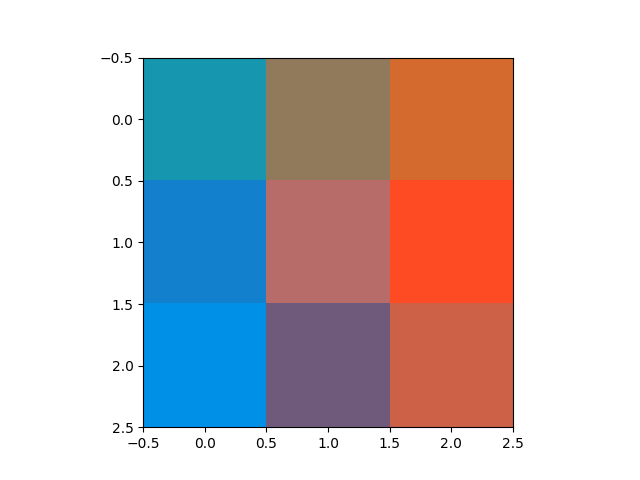
\includegraphics[width=0.125\textwidth]{filter0.png}}%
\subcaptionbox{filter 01}{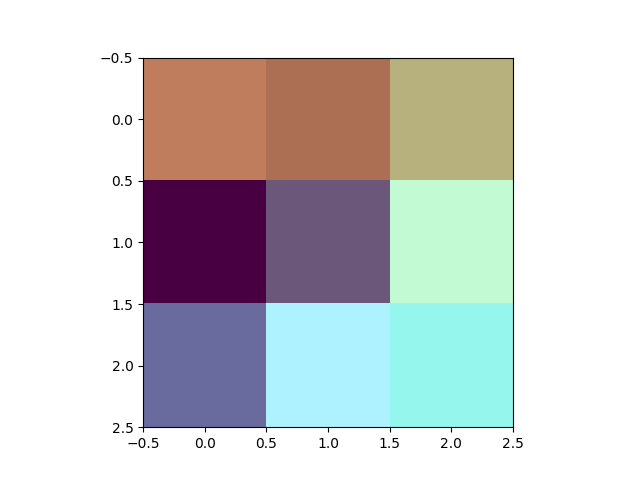
\includegraphics[width=0.125\textwidth]{filter1.png}}%
\subcaptionbox{filter 02}{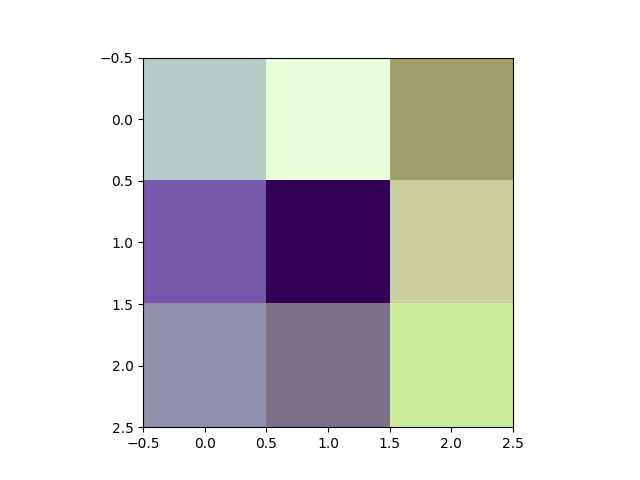
\includegraphics[width=0.125\textwidth]{filter2.png}}%
\subcaptionbox{filter 03}{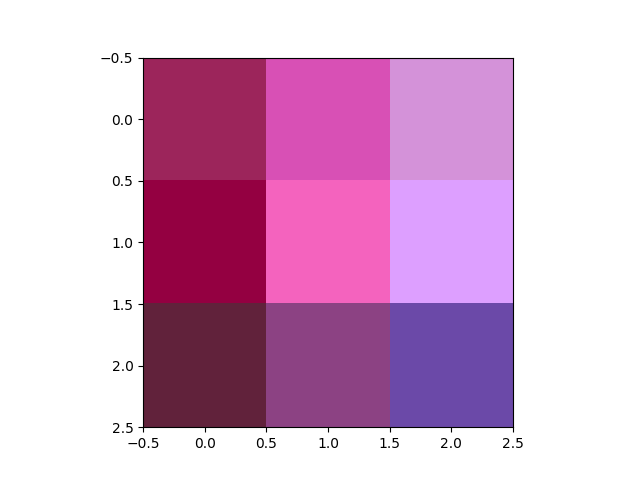
\includegraphics[width=0.125\textwidth]{filter3.png}}%
\subcaptionbox{filter 04}{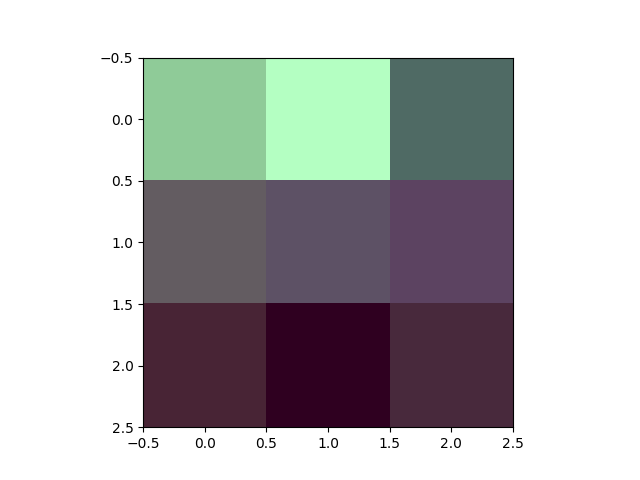
\includegraphics[width=0.125\textwidth]{filter4.png}}%
\subcaptionbox{filter 05}{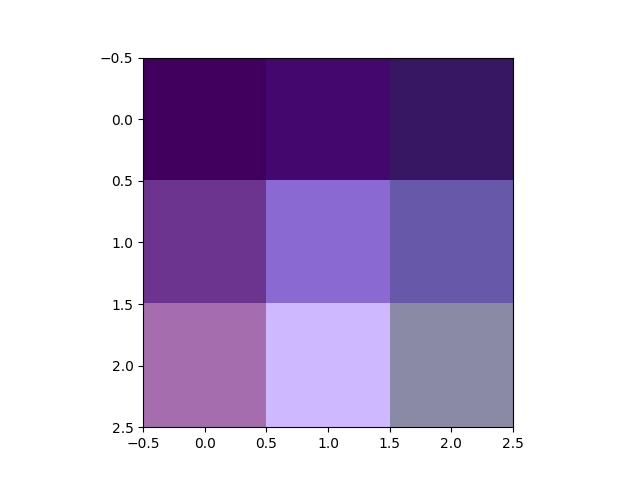
\includegraphics[width=0.125\textwidth]{filter5.png}}%
\subcaptionbox{filter 06}{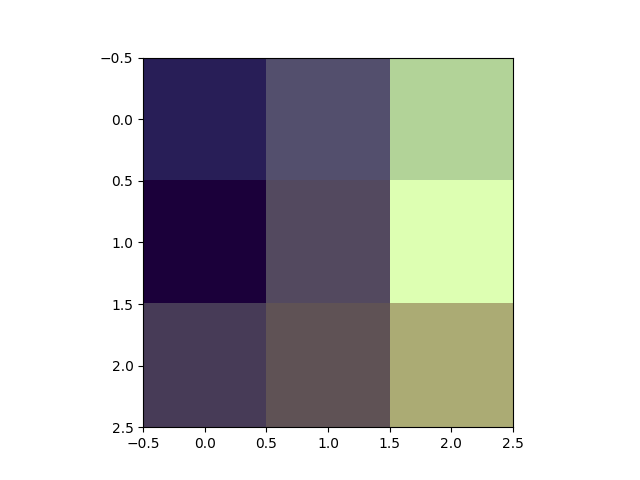
\includegraphics[width=0.125\textwidth]{filter6.png}}%
\subcaptionbox{filter 07}{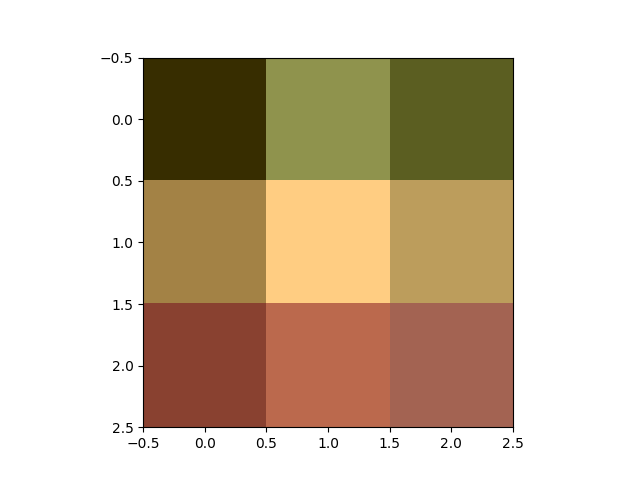
\includegraphics[width=0.125\textwidth]{filter7.png}}\\%

\subcaptionbox{filter 8}{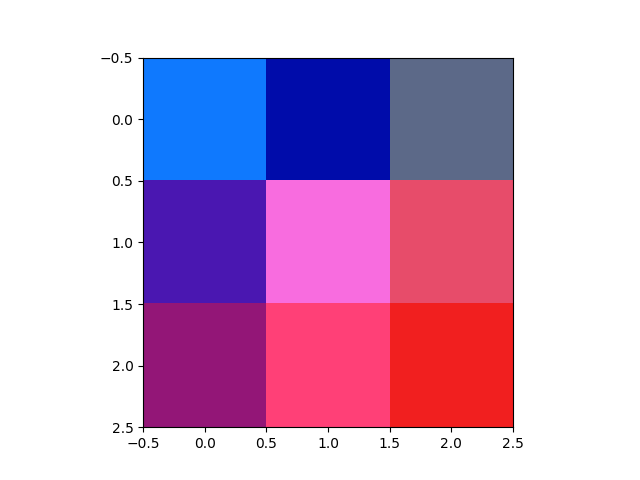
\includegraphics[width=0.125\textwidth]{filter8.png}}%
\subcaptionbox{filter 9}{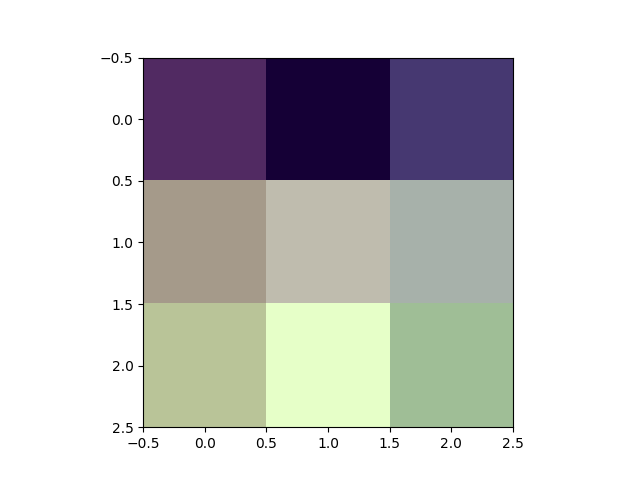
\includegraphics[width=0.125\textwidth]{filter9.png}}%
\subcaptionbox{filter 10}{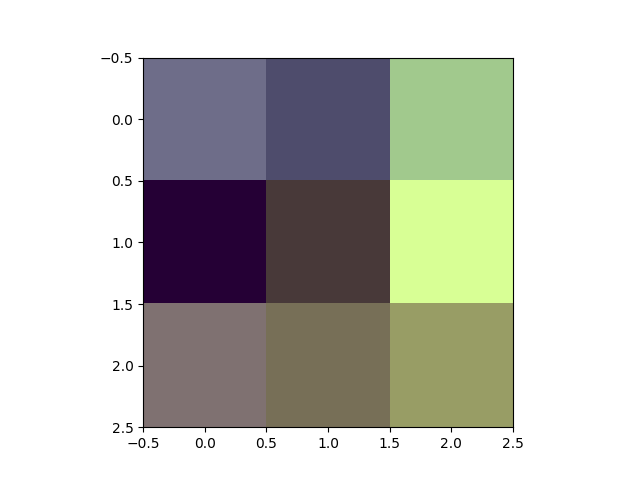
\includegraphics[width=0.125\textwidth]{filter10.png}}%
\subcaptionbox{filter 11}{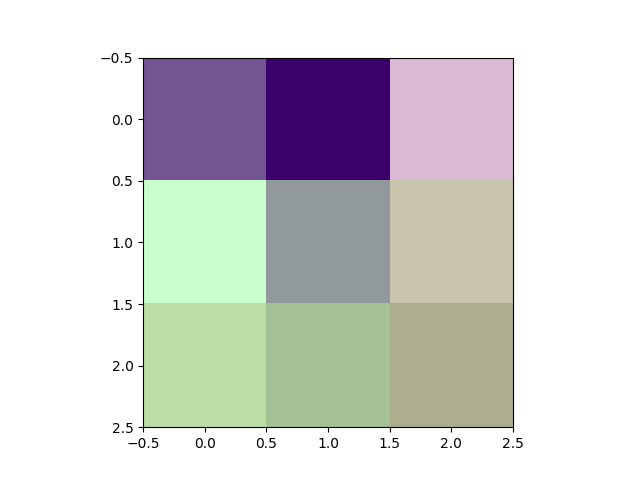
\includegraphics[width=0.125\textwidth]{filter11.png}}%
\subcaptionbox{filter 12}{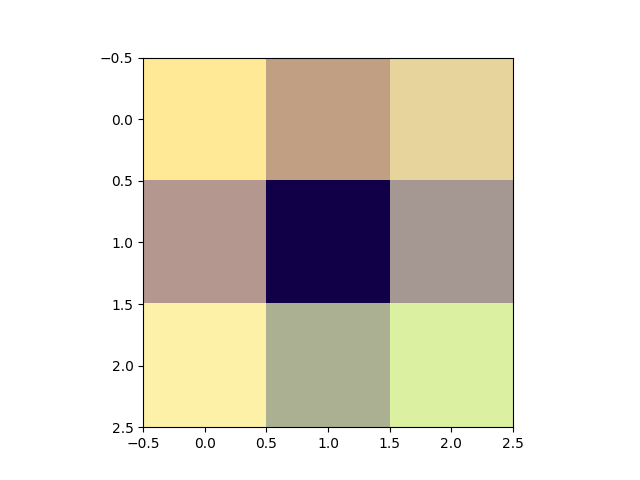
\includegraphics[width=0.125\textwidth]{filter12.png}}%
\subcaptionbox{filter 13}{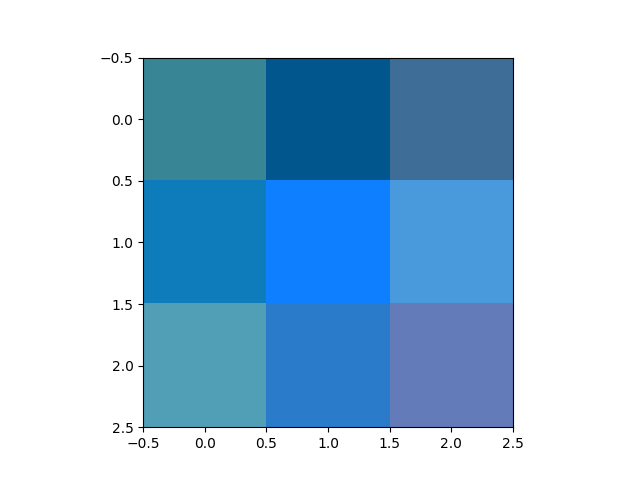
\includegraphics[width=0.125\textwidth]{filter13.png}}%
\subcaptionbox{filter 14}{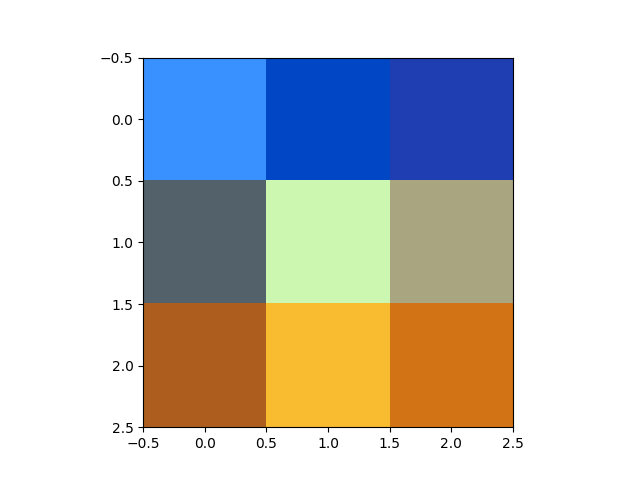
\includegraphics[width=0.125\textwidth]{filter14.png}}%
\subcaptionbox{filter 15}{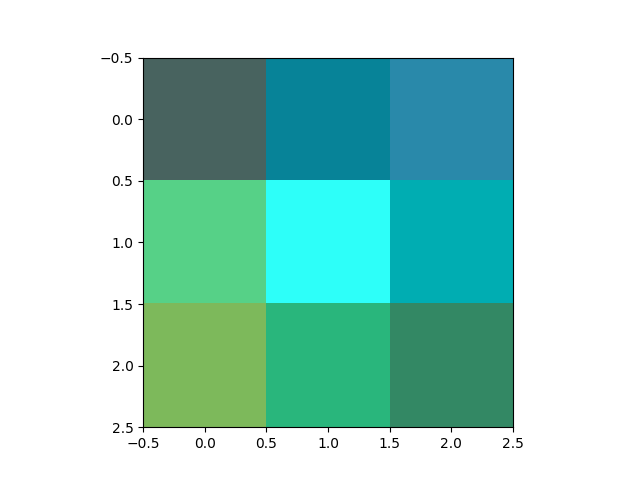
\includegraphics[width=0.125\textwidth]{filter15.png}}\\%

\subcaptionbox{filter 16}{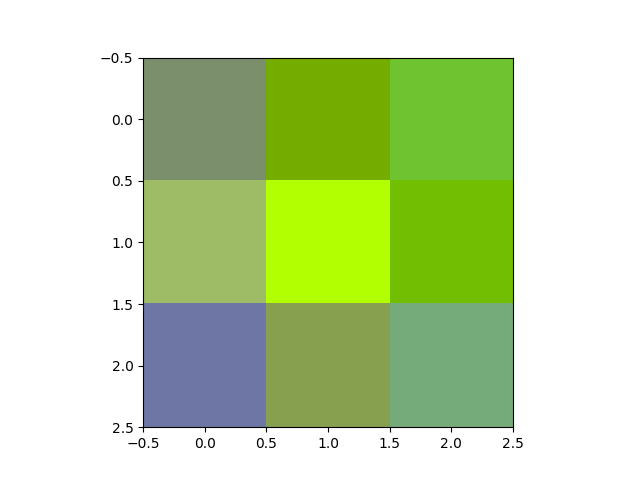
\includegraphics[width=0.125\textwidth]{filter16.png}}%
\subcaptionbox{filter 17}{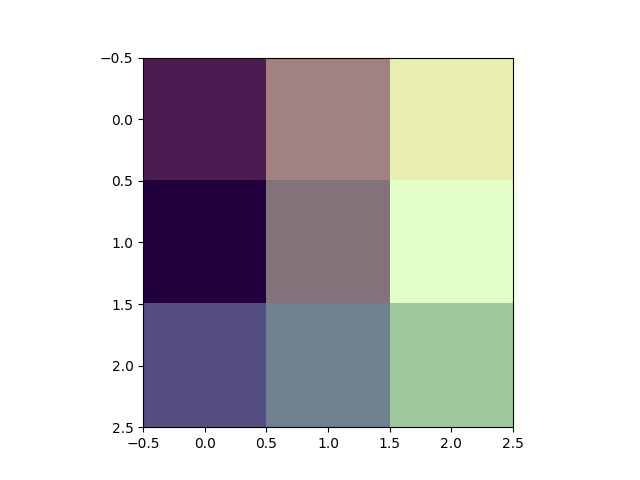
\includegraphics[width=0.125\textwidth]{filter17.png}}%
\subcaptionbox{filter 18}{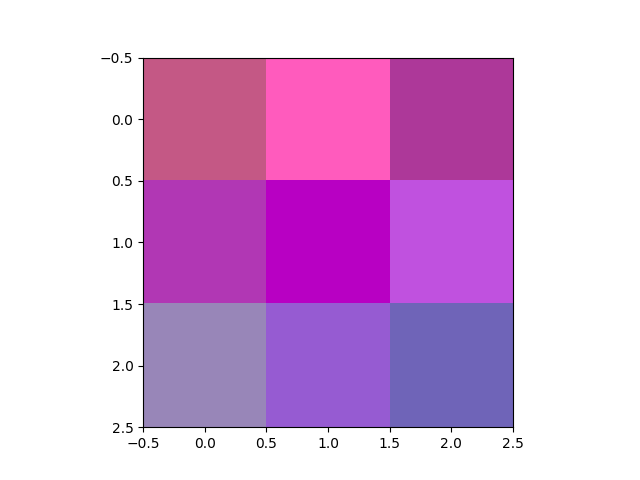
\includegraphics[width=0.125\textwidth]{filter18.png}}%
\subcaptionbox{filter 19}{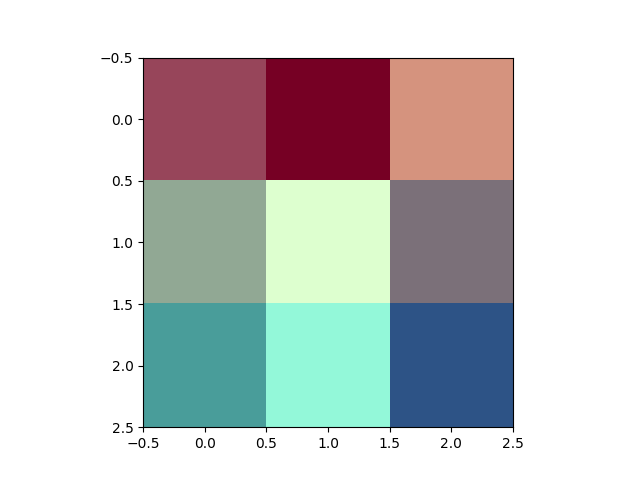
\includegraphics[width=0.125\textwidth]{filter19.png}}%
\subcaptionbox{filter 20}{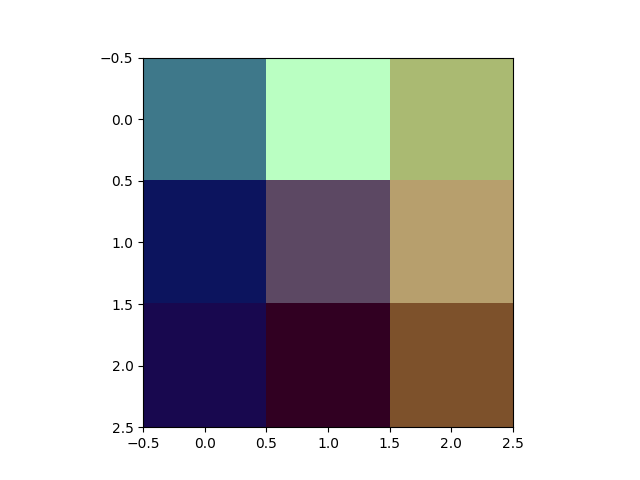
\includegraphics[width=0.125\textwidth]{filter20.png}}%
\subcaptionbox{filter 21}{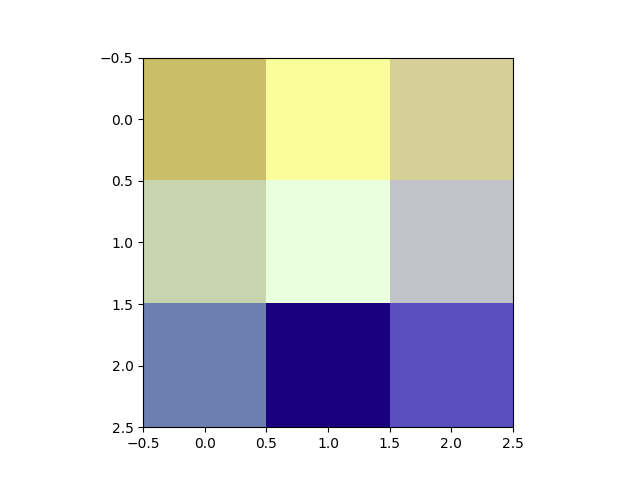
\includegraphics[width=0.125\textwidth]{filter21.png}}%
\subcaptionbox{filter 22}{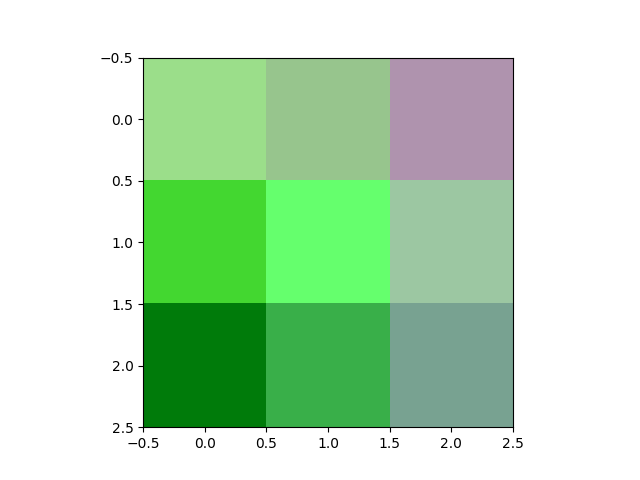
\includegraphics[width=0.125\textwidth]{filter22.png}}%
\subcaptionbox{filter 23}{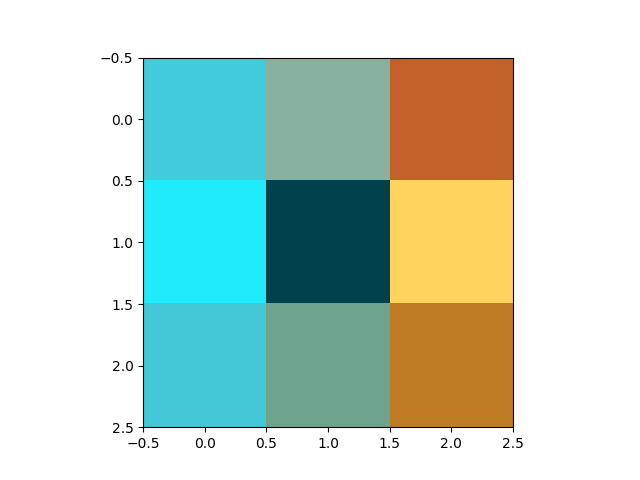
\includegraphics[width=0.125\textwidth]{filter23.png}}\\%

\subcaptionbox{filter 24}{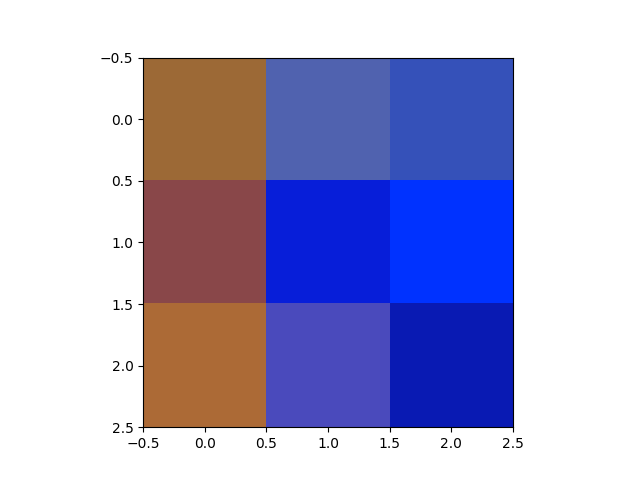
\includegraphics[width=0.125\textwidth]{filter24.png}}%
\subcaptionbox{filter 25}{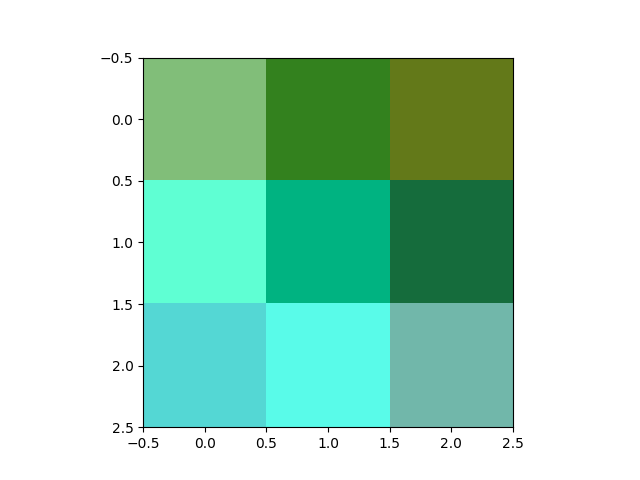
\includegraphics[width=0.125\textwidth]{filter25.png}}%
\subcaptionbox{filter 26}{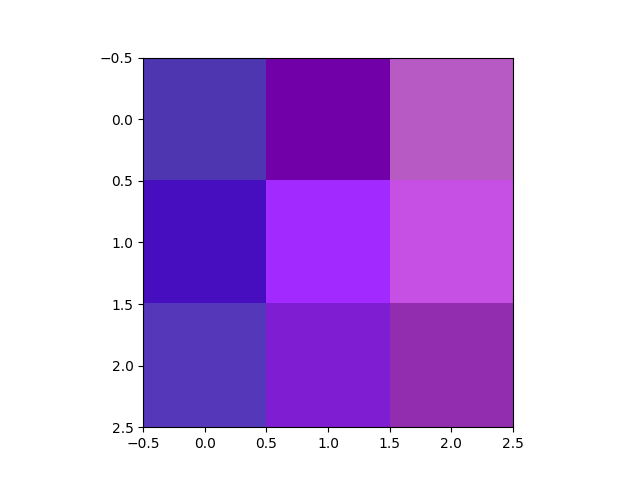
\includegraphics[width=0.125\textwidth]{filter26.png}}%
\subcaptionbox{filter 27}{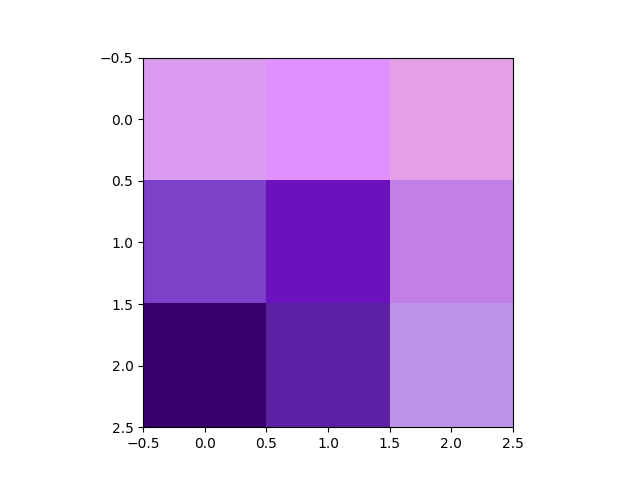
\includegraphics[width=0.125\textwidth]{filter27.png}}%
\subcaptionbox{filter 28}{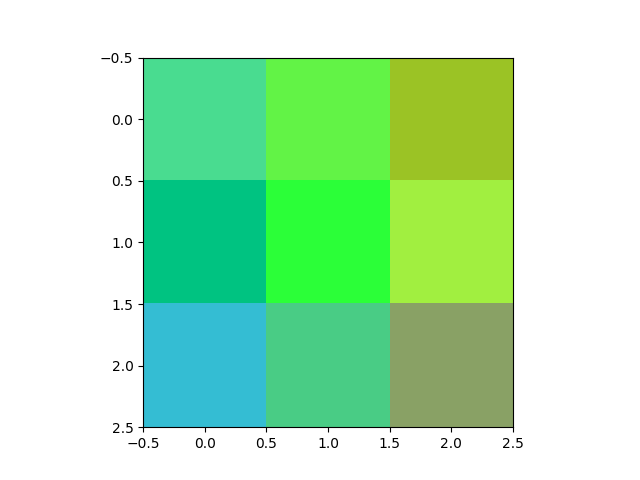
\includegraphics[width=0.125\textwidth]{filter28.png}}%
\subcaptionbox{filter 29}{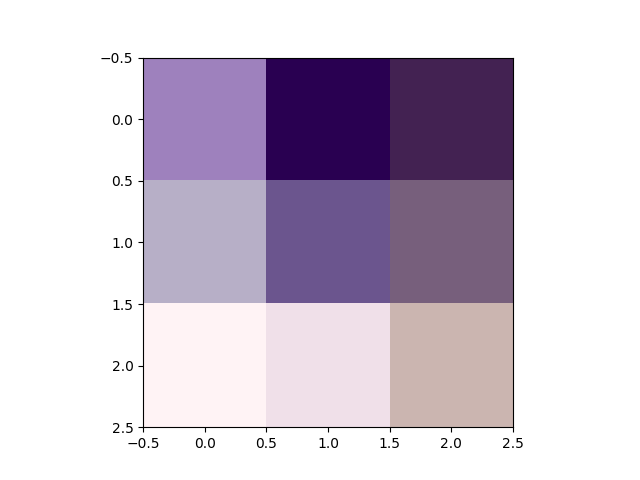
\includegraphics[width=0.125\textwidth]{filter29.png}}%
\subcaptionbox{filter 30}{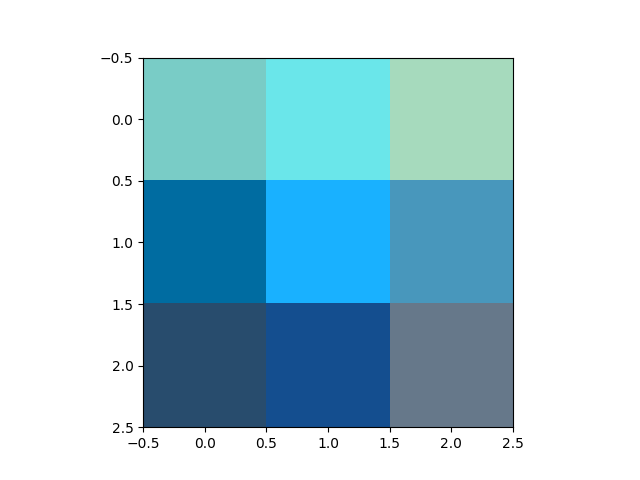
\includegraphics[width=0.125\textwidth]{filter30.png}}%
\subcaptionbox{filter 31}{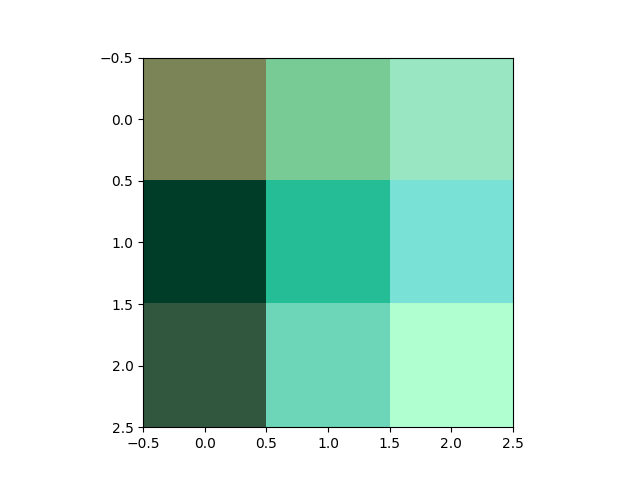
\includegraphics[width=0.125\textwidth]{filter31.png}}\\%

\subcaptionbox{filter 32}{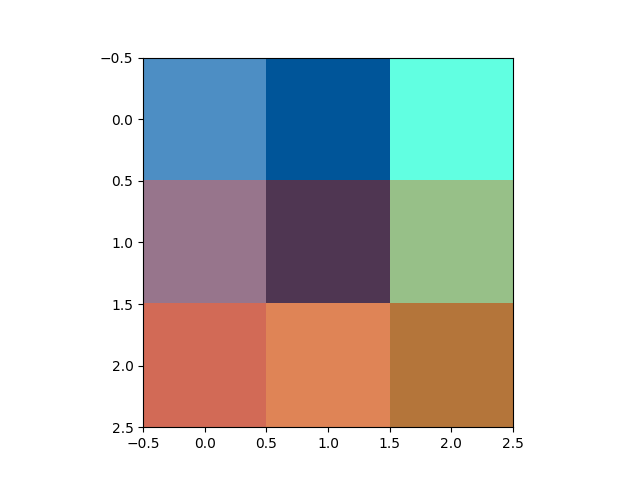
\includegraphics[width=0.125\textwidth]{filter32.png}}%
\subcaptionbox{filter 33}{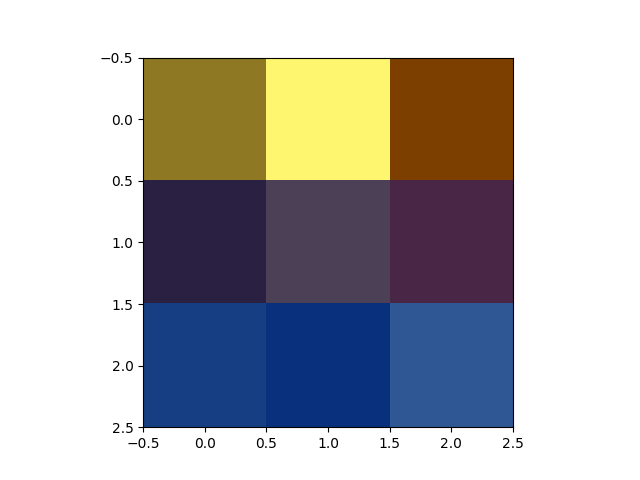
\includegraphics[width=0.125\textwidth]{filter33.png}}%
\subcaptionbox{filter 34}{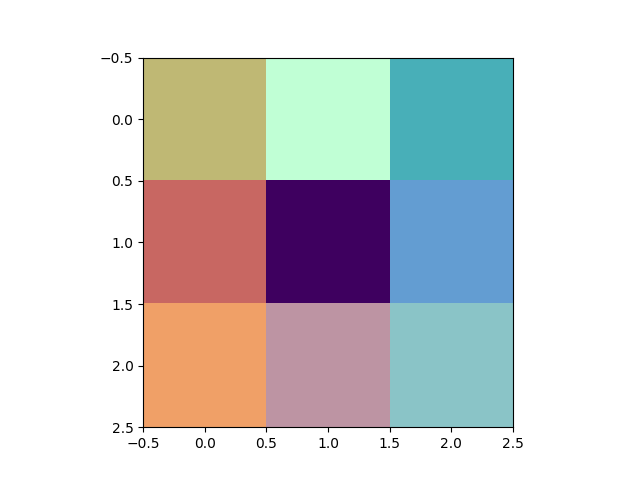
\includegraphics[width=0.125\textwidth]{filter34.png}}%
\subcaptionbox{filter 35}{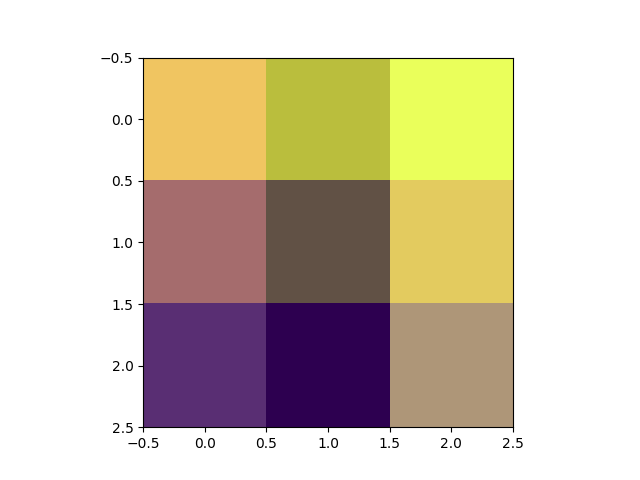
\includegraphics[width=0.125\textwidth]{filter35.png}}%
\subcaptionbox{filter 36}{\includegraphics[width=0.125\textwidth]{filter36.png}}%
\subcaptionbox{filter 37}{\includegraphics[width=0.125\textwidth]{filter37.png}}%
\subcaptionbox{filter 38}{\includegraphics[width=0.125\textwidth]{filter38.png}}%
\subcaptionbox{filter 39}{\includegraphics[width=0.125\textwidth]{filter39.png}}\\%

\subcaptionbox{filter 40}{\includegraphics[width=0.125\textwidth]{filter40.png}}%
\subcaptionbox{filter 41}{\includegraphics[width=0.125\textwidth]{filter41.png}}%
\subcaptionbox{filter 42}{\includegraphics[width=0.125\textwidth]{filter42.png}}%
\subcaptionbox{filter 43}{\includegraphics[width=0.125\textwidth]{filter43.png}}%
\subcaptionbox{filter 44}{\includegraphics[width=0.125\textwidth]{filter44.png}}%
\subcaptionbox{filter 45}{\includegraphics[width=0.125\textwidth]{filter45.png}}%
\subcaptionbox{filter 46}{\includegraphics[width=0.125\textwidth]{filter46.png}}%
\subcaptionbox{filter 47}{\includegraphics[width=0.125\textwidth]{filter47.png}}\\%

\subcaptionbox{filter 48}{\includegraphics[width=0.125\textwidth]{filter48.png}}%
\subcaptionbox{filter 49}{\includegraphics[width=0.125\textwidth]{filter49.png}}%
\subcaptionbox{filter 50}{\includegraphics[width=0.125\textwidth]{filter50.png}}%
\subcaptionbox{filter 51}{\includegraphics[width=0.125\textwidth]{filter51.png}}%
\subcaptionbox{filter 52}{\includegraphics[width=0.125\textwidth]{filter52.png}}%
\subcaptionbox{filter 53}{\includegraphics[width=0.125\textwidth]{filter53.png}}%
\subcaptionbox{filter 54}{\includegraphics[width=0.125\textwidth]{filter54.png}}%
\subcaptionbox{filter 55}{\includegraphics[width=0.125\textwidth]{filter55.png}}\\%

\subcaptionbox{filter 56}{\includegraphics[width=0.125\textwidth]{filter56.png}}%
\subcaptionbox{filter 57}{\includegraphics[width=0.125\textwidth]{filter57.png}}%
\subcaptionbox{filter 58}{\includegraphics[width=0.125\textwidth]{filter58.png}}%
\subcaptionbox{filter 59}{\includegraphics[width=0.125\textwidth]{filter59.png}}%
\subcaptionbox{filter 60}{\includegraphics[width=0.125\textwidth]{filter60.png}}%
\subcaptionbox{filter 61}{\includegraphics[width=0.125\textwidth]{filter61.png}}%
\subcaptionbox{filter 62}{\includegraphics[width=0.125\textwidth]{filter62.png}}%
\subcaptionbox{filter 63}{\includegraphics[width=0.125\textwidth]{filter63.png}}\\%
\caption{Filters in first conv layer}
\label{fig-filter-in1}
\end{figure}

\begin{figure}[H]
\centering
\subcaptionbox{filter 6 (blue line)}{\includegraphics[width=0.25\textwidth]{filter6.png}}%
\subcaptionbox{activation from filter 6}{\includegraphics[width=0.25\textwidth]{first_conv6.png}}%
\subcaptionbox{filter 27 (dark corner)}{\includegraphics[width=0.25\textwidth]{filter27.png}}%
\subcaptionbox{activation from filter 27}{\includegraphics[width=0.25\textwidth]{first_conv27.png}}\\%

\subcaptionbox{filter 15 (green surface)}{\includegraphics[width=0.25\textwidth]{filter15.png}}%
\subcaptionbox{activation from filter 15 }{\includegraphics[width=0.25\textwidth]{first_conv15.png}}%
\subcaptionbox{filter 47 (yellow surface)}{\includegraphics[width=0.25\textwidth]{filter47.png}}%
\subcaptionbox{activation from filter 47 }{\includegraphics[width=0.25\textwidth]{first_conv47.png}}%
\caption{Activations and corresponding filters in first conv layer}
\label{fig-filter-in}
\end{figure}

In general, activations from the filters indicate different convolutional layers in cascade  structured neural network model perform different tasks during the image classification process. The initial convolutional layers mainly focus on basic geometry features in image, like corners or lines. And the higher level convolutional layers tend to learn some semantic elements and components to help with image classification. The pixel level information is first transformed to lower level feature, then propagate to convolutional layers afterwards to higher level comprehension. And the diversity of filters in the first convolutional layers, both in color distribution and gradient of pixel intensity, guarantees that the information from the image can be maximum preserved and utilize to help downstream convolutional layers do the classfication.

\subsection{Feature Extraction}
In this section we are going to design experiement to illustrate how the depth of the convolutional neural network decides the classification performance. 

\subsubsection{Experiment Setup}
Here we reserved the former structure of the transfered-VGG16 net, and altered the two-layer fully connection layer to a single hidden layer with 1000 hidden units. The final layer is still kept as a softmax layer with 256 dimension output. The original VGG16 net has 5 convolutional blocks. We used the first 3, 4 and all 5 convolutional blocks respectively and calculated the classfication metrics. To get best accuracy in each cases, our learning rate is set as 0.0005 for 4 and 5 conv blocks, and 0.0001 for 3 conv blocks. Our annealing factor $T$ is set as 50. All other parameters are the same mentioned in Table \ref{tab-trans1}. We use the result from transfer learning part as our baseline.

\subsubsection{Discussion}
Different performances by using different numbers of conv blocks are shown in Table \ref{tab-cmp}. Here "i-conv" means using i conv blocks for classification, and "conv-i" means the i-th conv block in VGG16. We can see that using only part of (conv blocks of) pre-trained VGG model also can do the classification job, but in a very low accuracy. As the conv blocks numbers increasing, the accuracy increases sharply, from 29.74\% to 71.29\%. While adding another hidden layer or increasing the hidden units numbers don't improve the performance too much, just by several percentages. Also we can see that during training phase, the accuracy on training set of shallower model tends to reach closer to 1. This is because although the number of layers is less, the scale of output features from the last conv block is much bigger ($28\times 28\times 256=200704$ in 3-conv case) than the ($7\times 7\times 512=25088$ in 5-conv case) which result in more number of weighs in fully connected layer. And because we only have limited number of data on Caltech-256(30607 images), we can easily get overfit.

\begin{table}[H]
	\caption{Accuracy Comparison}
	\centering
	\begin{tabular}{|c|c|c|c|c|}
		\hline
		 & 3-conv & 4-conv & 5-conv & baseline\\
		\hline
		level-1 & conv-1   & conv-1   & conv-1   & conv-1\\
		\hline
		level-2 & conv-2   & conv-2   & conv-2   & conv-2\\
		\hline
		level-3 & conv-3   & conv-3   & conv-3   & conv-3\\
		\hline
		level-4 & fc(1000) & conv-4   & conv-4   & conv-4\\
		\hline
		level-5 & softmax  & fc(1000) & conv-5   & conv-5\\
        \hline
		level-6 &          & softmax  & fc(1000) & fc(4096)\\		
		\hline
		level-7 &          &          & softmax  & fc(4096)\\
		\hline
		level-8 &          &          &          & softmax\\
		\hline
		Train acc. &1.0000 & 1.0000   & 0.9993   & 0.9500 \\
		\hline
		Valid acc. &0.2822 & 0.5166   & 0.7129   & 0.7100 \\
		\hline		
		Test acc.  &0.2876 & 0.5322   & 0.7129   & 0.7554 \\
		\hline		
	\end{tabular}
	\label{tab-cmp}
\end{table}